\chapter{Example mesh and elements}

To illustrate the relationship between control points and their
association with individual elements defined by knot spacing we show
a few two-dimensional examples.

\begin{quote}
\noindent
\textbf{Example: 2-d NURBS patch of quadratic elements}

The mesh and elements for a $3 \times 3$ patch of quadratic elements is
shown in Fig. \ref{fig5ex1}.  The individual elements of the mesh and
their associated control points are shown in Fig. \ref{fig5ex2}.

\begin{figure}[!h]
\begin{center}

\centerline{
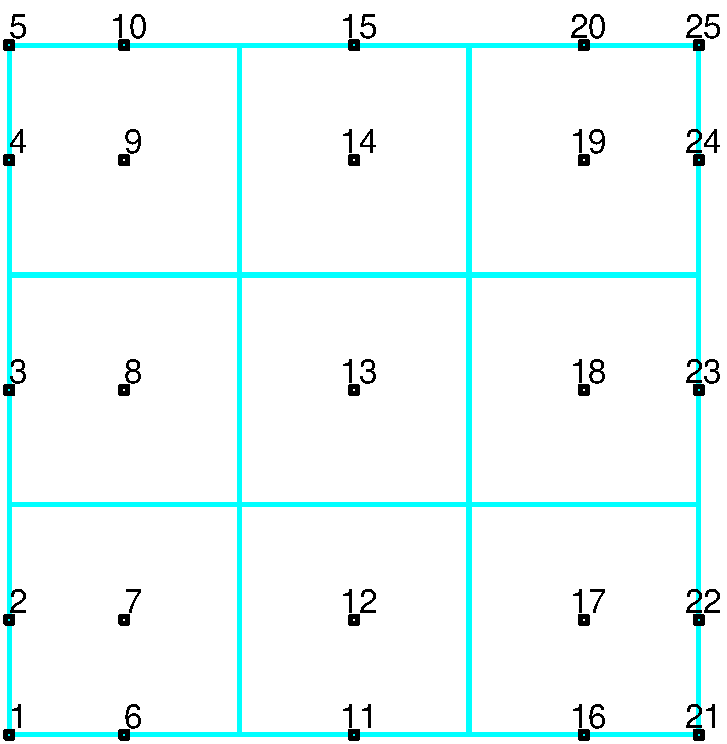
\includegraphics[width=2.8in]{figs/mesh_2d} \hspace{0.2in}
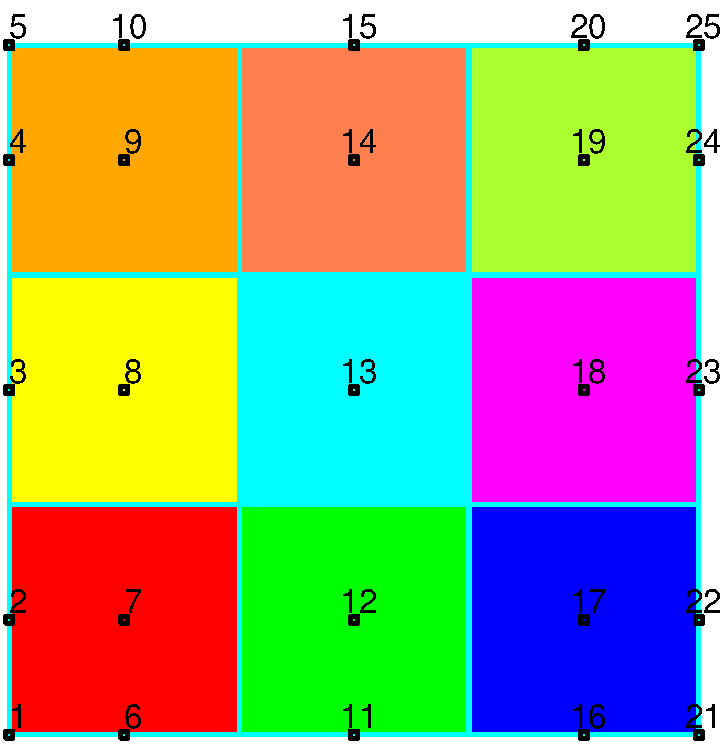
\includegraphics[width=2.8in]{figs/mesh_fill}
}

\centerline{(a) Mesh with control points \hspace{1in} (b) Elements in color}

\caption{Two dimensional NURBS patch of quadratic elements.  \label{fig5ex1}}
\end{center}
\end{figure}

\begin{figure}[!h]
\begin{center}

\centerline{
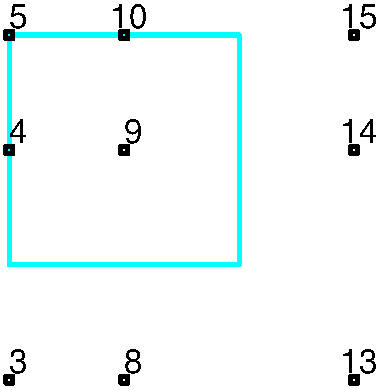
\includegraphics[width=1.2in]{figs/mesh_e7} \hspace{0.2in}
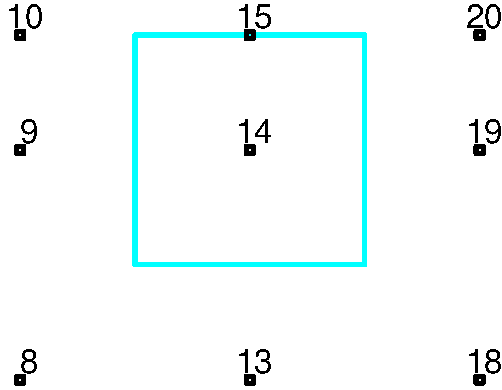
\includegraphics[width=1.6in]{figs/mesh_e8} \hspace{0.2in}
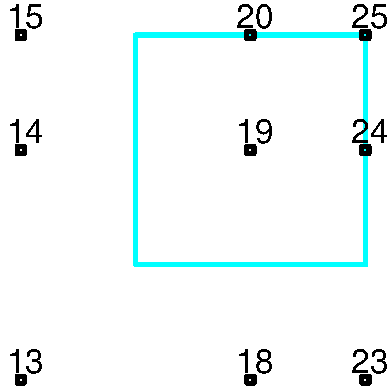
\includegraphics[width=1.2in]{figs/mesh_e9}
}

\centerline{(i) Element 7 \hspace{0.7in} (j) Element 8 \hspace{0.7in} (k) Element 9}

\centerline{
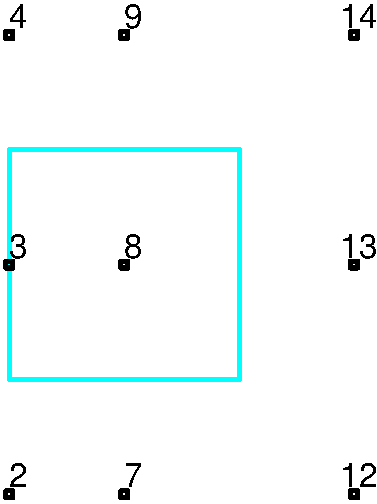
\includegraphics[width=1.2in]{figs/mesh_e4} \hspace{0.2in}
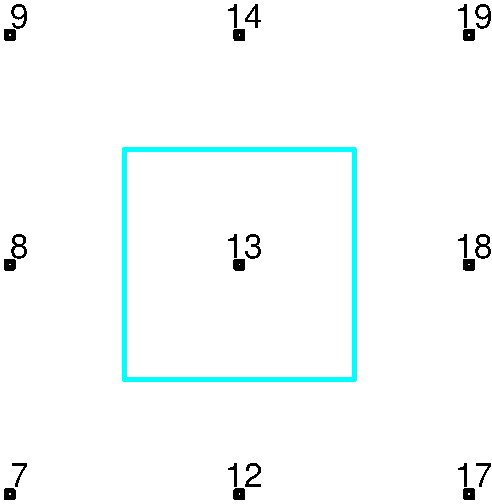
\includegraphics[width=1.6in]{figs/mesh_e5} \hspace{0.2in}
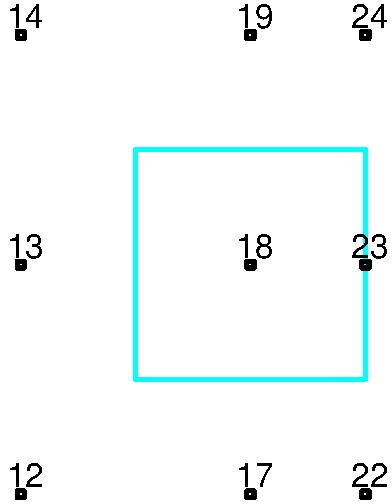
\includegraphics[width=1.2in]{figs/mesh_e6}
}

\centerline{(d) Element 4 \hspace{0.7in} (e) Element 5 \hspace{0.7in} (f) Element 6}

\centerline{
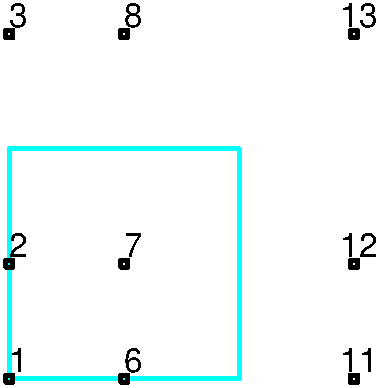
\includegraphics[width=1.2in]{figs/mesh_e1} \hspace{0.2in}
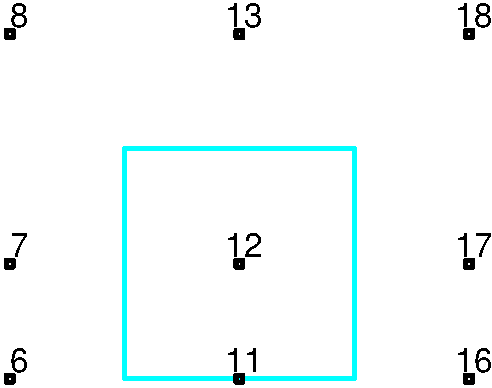
\includegraphics[width=1.6in]{figs/mesh_e2} \hspace{0.2in}
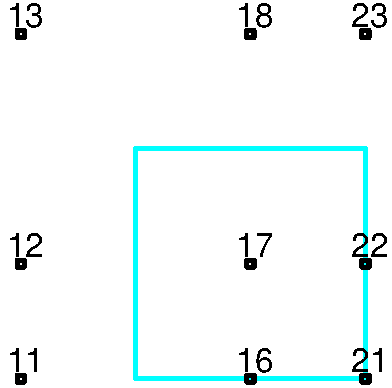
\includegraphics[width=1.2in]{figs/mesh_e3}
}

\centerline{(a) Element 1 \hspace{0.7in} (b) Element 2 \hspace{0.7in} (c) Element 3}

\caption{Individual elements for 2-d NURBS patch of quadratic elements.  \label{fig5ex2}}
\end{center}
\end{figure}

\end{quote}

\begin{quote}
\noindent
\textbf{Example: 2-d NURBS patch of cubic elements}

The mesh and elements for a $3 \times 3$ patch of cubic elements is
shown in Fig. \ref{fig5ex3}.  The individual elements of the mesh and
their associated control points are shown in Fig. \ref{fig5ex4}.

\begin{figure}[!t]
\begin{center}

\centerline{
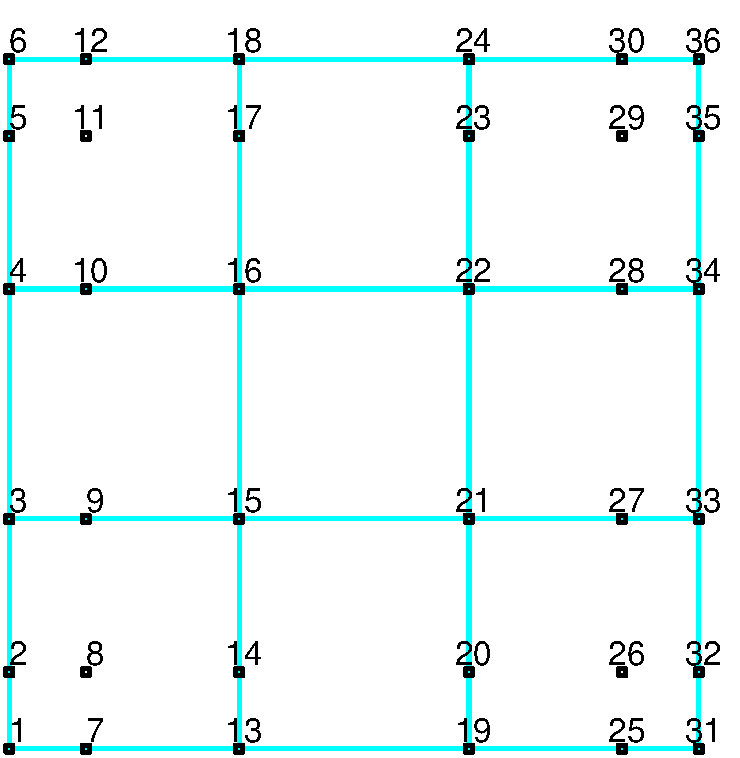
\includegraphics[width=2.0in]{figs/mesh_3_mesh} \hspace{0.2in}
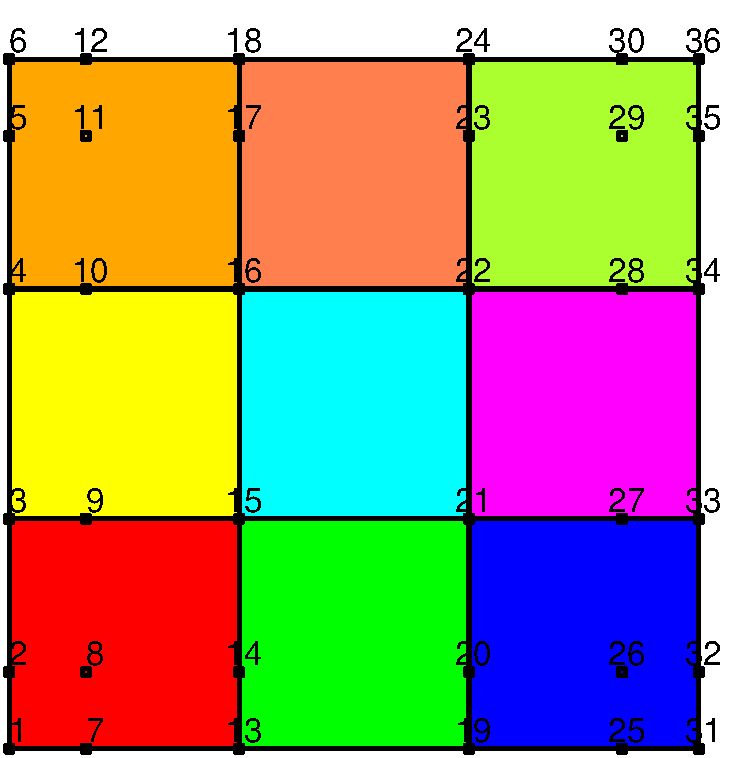
\includegraphics[width=2.0in]{figs/mesh_3_fill}
}

\centerline{(a) Mesh with control points \hspace{1in} (b) Elements in color}

\caption{Two dimensional NURBS patch of cubic elements.  \label{fig5ex3}}
\end{center}
\end{figure}

\begin{figure}[!b]
\begin{center}

\centerline{
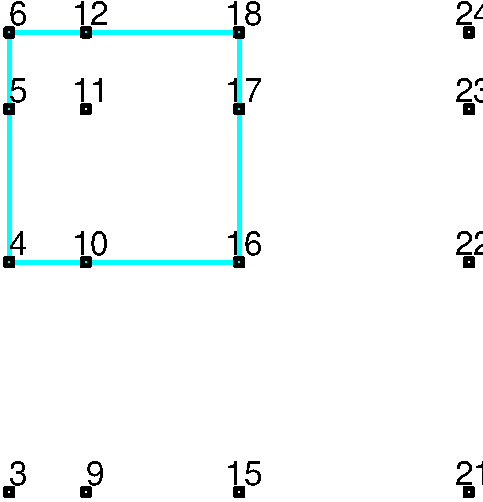
\includegraphics[width=1.2in]{figs/mesh_3_e7} \hspace{0.2in}
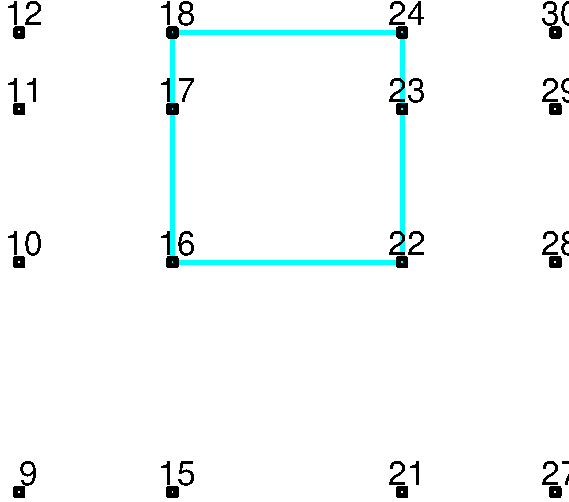
\includegraphics[width=1.4in]{figs/mesh_3_e8} \hspace{0.2in}
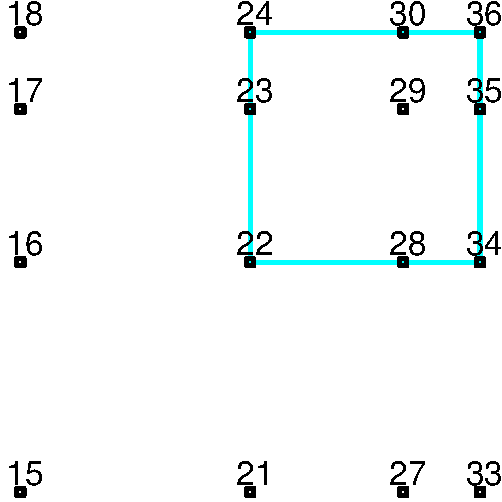
\includegraphics[width=1.2in]{figs/mesh_3_e9}
}

\centerline{(i) Element 7 \hspace{0.7in} (j) Element 8 \hspace{0.7in} (k) Element 9}

\centerline{
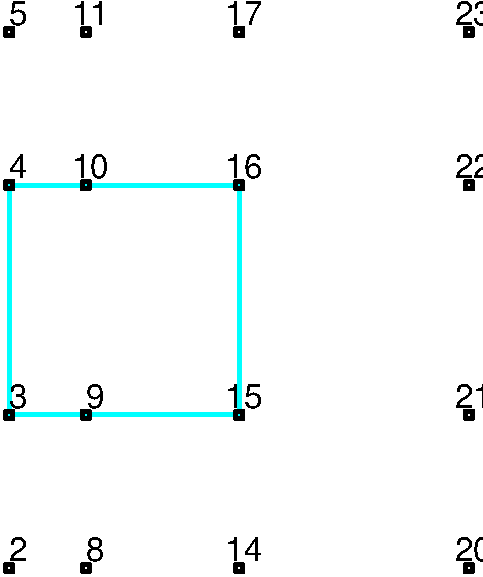
\includegraphics[width=1.2in]{figs/mesh_3_e4} \hspace{0.2in}
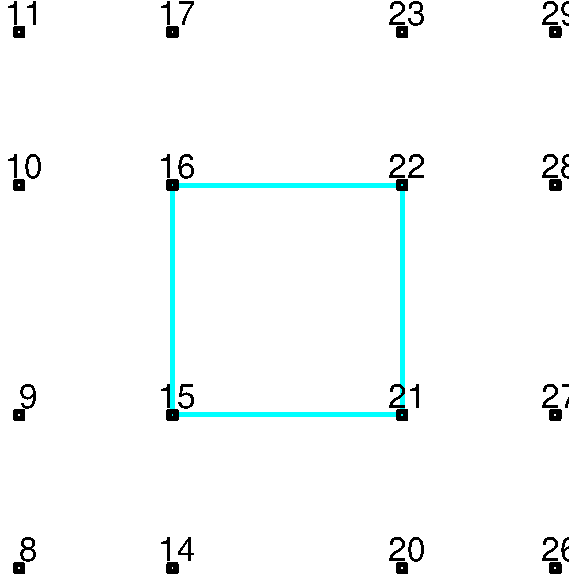
\includegraphics[width=1.4in]{figs/mesh_3_e5} \hspace{0.2in}
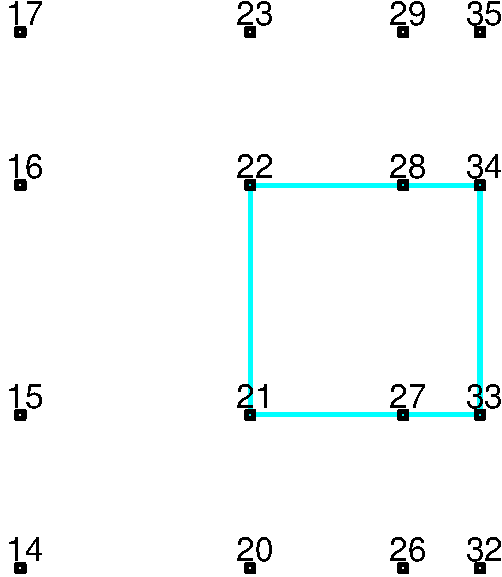
\includegraphics[width=1.2in]{figs/mesh_3_e6}
}

\centerline{(d) Element 4 \hspace{0.7in} (e) Element 5 \hspace{0.7in} (f) Element 6}

\centerline{
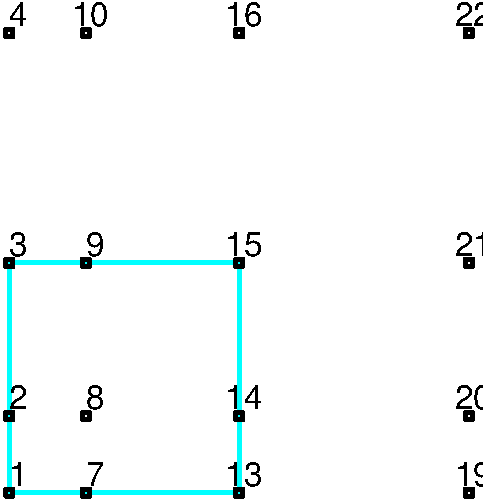
\includegraphics[width=1.2in]{figs/mesh_3_e1} \hspace{0.2in}
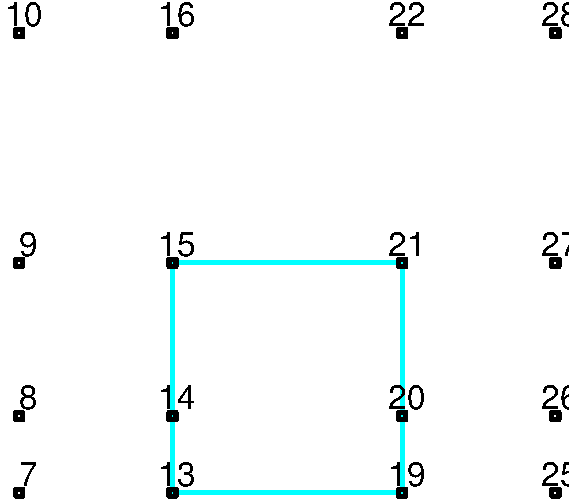
\includegraphics[width=1.4in]{figs/mesh_3_e2} \hspace{0.2in}
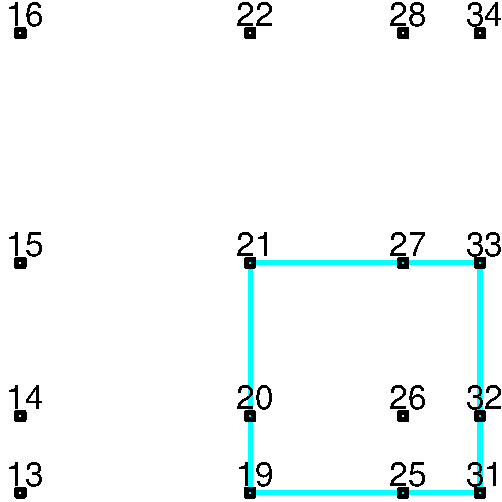
\includegraphics[width=1.2in]{figs/mesh_3_e3}
}

\centerline{(a) Element 1 \hspace{0.7in} (b) Element 2 \hspace{0.7in} (c) Element 3}

\caption{Individual elements for 2-d NURBS patch of cubic elements.  \label{fig5ex4}}
\end{center}
\end{figure}

\end{quote}

\begin{quote}
\noindent
\textbf{Example: 2-d NURBS patch of quartic elements}

The mesh and elements for a $3 \times 3$ patch of quartic elements is
shown in Fig. \ref{fig5ex5}.  The individual element description is not
shown, however, each element involves a $5 \times 5$ patch of control
point which
overlap between elements except for one control point.  Thus, the mesh only grows
by one control point in each direction as the order is increased.

\begin{figure}[!t]
\begin{center}

\centerline{
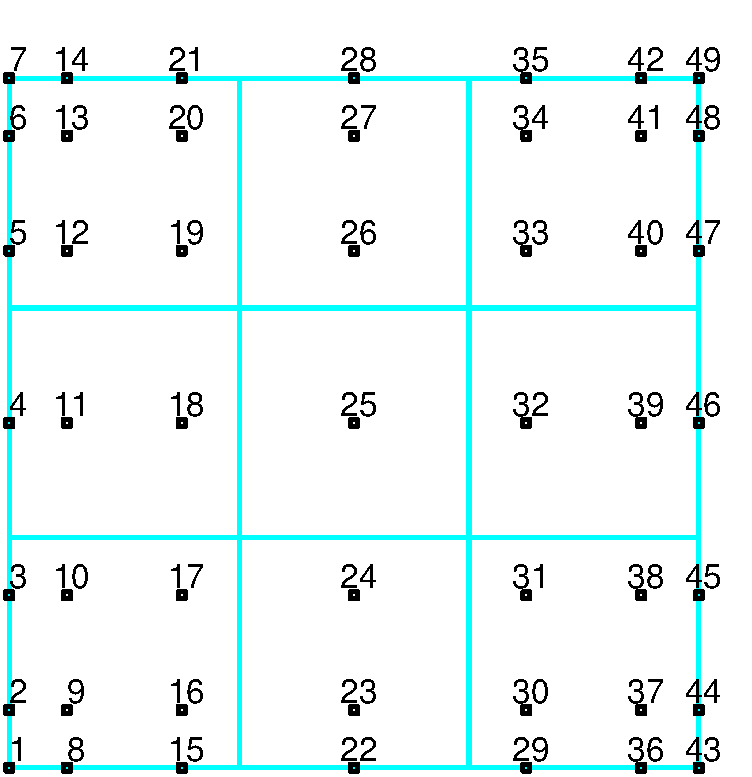
\includegraphics[width=2.0in]{figs/mesh_4_mesh} \hspace{0.2in}
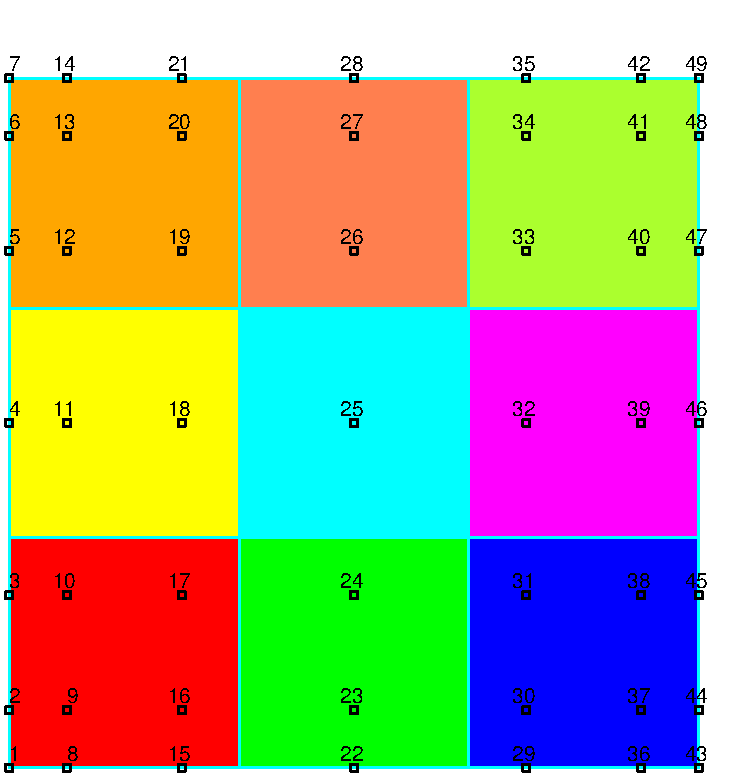
\includegraphics[width=2.0in]{figs/mesh_4_fill}
}

\centerline{(a) Mesh with control points \hspace{1in} (b) Elements in color}

\caption{Two dimensional NURBS patch of quartic elements.  \label{fig5ex5}}
\end{center}
\end{figure}
\end{quote}
